% \setchapterstyle{kao}
\setchapterimage{chargers-title3}
% \setchapterpreamble[u]{\margintoc}
\chapter{Data}
\label{ch:data}

\footnotetext{Title image is a map o f Prague with all chargers denoted as triangles in available datasets. The layer below displays all buildings in Prague with color being the number of floors}




In this chapter types data will be introduced, how they are classified and data formats in which they were obtained. Chargers, charging session dat and some lightweitght ontology will be described. Then followed with transformations of charging sessions into \acrfull{APC} which will be target variable in our model.

Then data that are considered and used to predict \acrfull{APC} will be introduced together with their transformation into a desirable form for our model.

Some of the data have not been used \sidenote{The inclusion of these data did not lead to lower validation loss of our model} but are part of data landscape considered and hold usefull information on what was thought might have an effect but in fact did not have.

\section{Types of data}

\begin{itemize}
    \item \textbf{spatial}(geospatial) data are those which have assigned position in real world and are invariant in some timeframe \sidenote{Nothing is permanent but in the time window of this thesis they have been invarinat}. Such data are locations of \acrfull{CS}, administrative boundaries, road network, buildings.
    \item \textbf{temporal} data are characterized by their variation over time without specific geographical coordinates. In this study, these include charging session durations, energy consumption patterns throughout the day, historical charger utilization rates, and seasonal variations in charging demand.
    \item \textbf{spatio-temporal} data incorporate both location and time elements, providing insights into how phenomena evolve across space and time. Examples relevant to this research include mobility patterns of people, real-time charger availability, and dynamic variations in \acrshort{APC} across different city zones during different hours of the day.
\end{itemize}

\section{EV Chargers and Charging Sessions}


\begin{figure}[hb]
    \includegraphics[width=1\textwidth]{data/charger-ontology.png}
    \caption{A charging ontology}
    \label{fig:charging-ontology}
\end{figure}


To introduce our problem domain and a possiblity to connect the data and how they relate. An simple charger ontology is introduced \sidenote{Ontology describe subjects of some system and a way how they are related together.}. Inspired by AURORAL EV-charger Ontology \sidecite{OntologyDocumentationGenerated} an ontolgoy of EV charging is introduced. The scope of it is to aide in understanding of the domain in this thesis.

The model matches data obtained from PRE.

Below is description of individual parts of the charging ontology as visible in \ref{fig:charging-ontology}.


\textbf{\acrlong{CS}} (as visible in \ref{fig:charging-station}) is equipment that connects an \acrshort{EV} to a source of electricity to recharge them. A charging station typically consists of physical infrastructure including power conversion hardware, connectivity modules, authentication systems, and user interfaces. Charging stations vary in their power delivery capabilities, ranging from slow AC chargers (3.7-22 kW) commonly found in residential and workplace settings to fast DC chargers (50-350+ kW) deployed in public corridors and commercial hubs. Within our dataset, charging stations from PRE's network predominantly consist of public AC and DC installations distributed throughout Prague's urban and suburban areas.

\begin{marginfigure}[]
    \centering
    \includegraphics[width=0.42\textwidth]{data/charger.png}
    \caption{Picture of \acrlong{CS}. It has one connector on each of its sides. One of which has charging cable attached.}
    \label{fig:charging-station}
\end{marginfigure}


\textbf{\acrlong{CP}} (as visible in \ref{fig:charging-connector}) one or many are part of a \acrshort{CS}. These physical interfaces allow for the actual connection between the vehicle and the charging infrastructure. Connectors follow different standards depending on region and charging speeds. Each connector type supports specific charging protocols and power levels. In our studied network, the majority of charging stations feature multiple connectors (typically two to four), enabling simultaneous charging of different vehicles and supporting various connector standards to accommodate the heterogeneous EV market.
\begin{marginfigure}[]
    \centering
    \includegraphics[width=0.3\textwidth]{data/charger-conector.png}
    \caption{View of 1 of the 2 charging connectors the \acrshort{CS} has}
    \label{fig:charging-connector}
\end{marginfigure}

\textbf{\acrlong{CSS}} occurs when an \acrshort{EV} arrives at a \acrshort{CS} and connects to a \acrshort{CP}. This interaction initiates a session that is logged by the \acrshort{CS} together with various parameters including connection time, disconnection time and total power consumed. The charging session represents the fundamental unit of analysis in our study, as it captures both temporal patterns (duration, time of day, day of week) and energy consumption behaviors. Our dataset contains records of these sessions across PRe chargers Prague's charging network over a multi-year period.

\textbf{location} denotes the geographical position where the charger is installed. This spatial attribute is helpfull to our analysis framework as it allows for correlation between charging demand and various features of the surrounding environment.

\subsection{Power consumption assumption}

Before we describe how \acrfull{CSS} have been processed into \acrlong{HPC} and \acrlong{APC}. In our model, we take simplyfing assumption on how actual power consumed during chargins session is consumed. Since actual power consumed can vary during charging of the electric vehicle. Most important is, the vehicle from connection time is being charged with the maximum power the \acrlong{EV} can handle and \acrlong{CP} can provide. This leads to charging session being split into two parts. First is charging part, that is when power is being delivered to the vehicle. And idle period where the vehicle has been fully charged and no power is being consumed\sidenote{Some charging station providers financially penalize this period of time, as an other \acrshort{EV} could have been charging. This can lead to improved availabilty of \acrlong{CS}.}



\begin{marginfigure}
    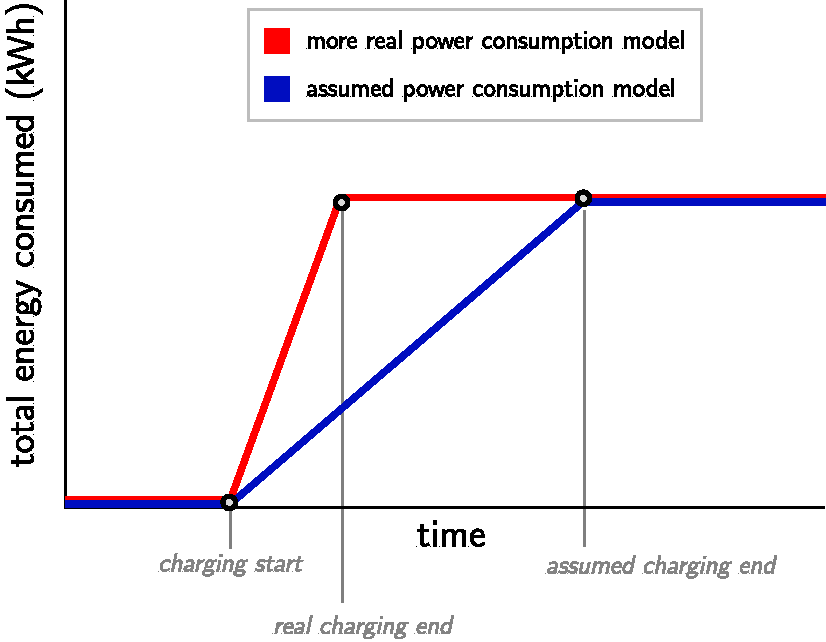
\includegraphics{charging-assumption.pdf}
    % \caption[Problem modelling overview]{Chapter content overview. }
\end{marginfigure}

\section{Population numbers (ZSJ)}

\begin{figure}[hb]
    \includegraphics{zsj-type.png}
    % \caption[Problem modelling overview]{Chapter content overview. }
\end{figure}

\section{Points of Interest}


\section{People Mobility}

\begin{figure}[hb]
    \includegraphics{commuting-people.png}
    \caption[Problem modelling overview]{Chapter content overview. }
\end{figure}

\section{Mobility Survey - cesko v pohybu}

\begin{figure}[hb]
    \includegraphics{vpohybu-trasnport-type.png}
    \caption[Problem modelling overview]{Chapter content overview. }
\end{figure}

---

Talks about what was extracted from datasets in \ref{ch:data}

\section{Spatial data}

\subsection{ZSJ Type and Population}

\subsection{Points of Interest}

Has statistically significant results for certain PoI \cite{hechtGlobalElectricVehicle2024}\cite{dongElectricVehicleCharging2019}
(\cite{dongElectricVehicleCharging2019} uses Gaussian cox model, \cite{hechtGlobalElectricVehicle2024} uses Neural networks and linear regression)

\cite{hechtGlobalElectricVehicle2024} states that radius of relevant PoIs is 2000metres. The research stated that the distance is sensible.
One solution is to just count all the PoIs in the radius but as they are more far away from the CP their relevance might decrease. The \cite{hechtGlobalElectricVehicle2024} thus uses importance factor for pair of PoI and CP.

$IF(PoI_i, CP_k) = max(r-d_{\text{sphere}}(PoI_i, CP_k),0)$


\subsubsection{Buildings (OsmPoisPbf)}


\subsubsection{Public Ammenities (OSMOX)}

how osmox works
\begin{figure}[hb]
    \includegraphics[width=0.7\textwidth]{osmox-poi.png}
    \caption[osmox]{osmox}
    \label{fig:nn-latent}
\end{figure}


\section{Charging profiles}


\begin{figure}[hb]
    \includegraphics[width=0.7\textwidth]{cutting-1.pdf}
    % \caption[Cutting]{Cutting}
\end{figure}

\begin{figure}[hb]
    \includegraphics[width=0.7\textwidth]{cutting-2.pdf}
    % \caption[Cutting]{Cutting}
\end{figure}


\section{}